\subsubsection{30.01.2016}
\textit{\textbf{Time frame:}} 16:00-21:30

The borders for debris were installed at both sides of the gripper (figure \ref{Gripper2.4}, \ref{Gripper2.5}). The extension of these borders was installed at both sides of the bucket (figure \ref{Gripper2.6}).

The moving mounts of the ribs were finished (figure \ref{Elevator3.8}).

\begin{figure}[H]
	\begin{minipage}[h]{0.47\linewidth}
		\center{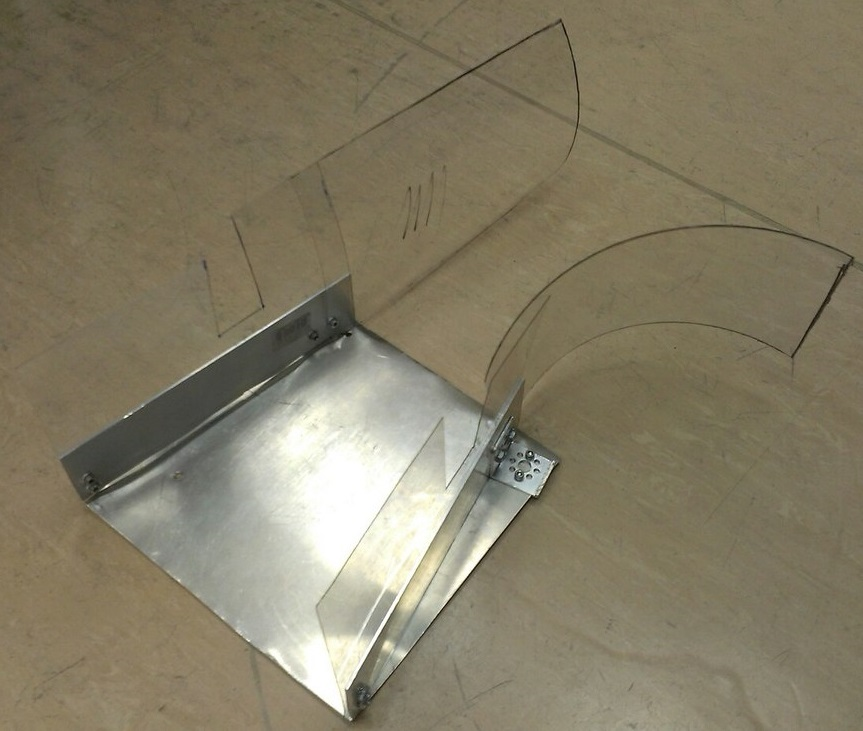
\includegraphics[scale=0.17]{3Engineering/5Team_meetings/days_of_meetings/2016.01.30/images/01}}
		\caption{Borders for debris}
		\label{Gripper2.4}
	\end{minipage}
	\hfill
	\begin{minipage}[h]{0.47\linewidth}
		\center{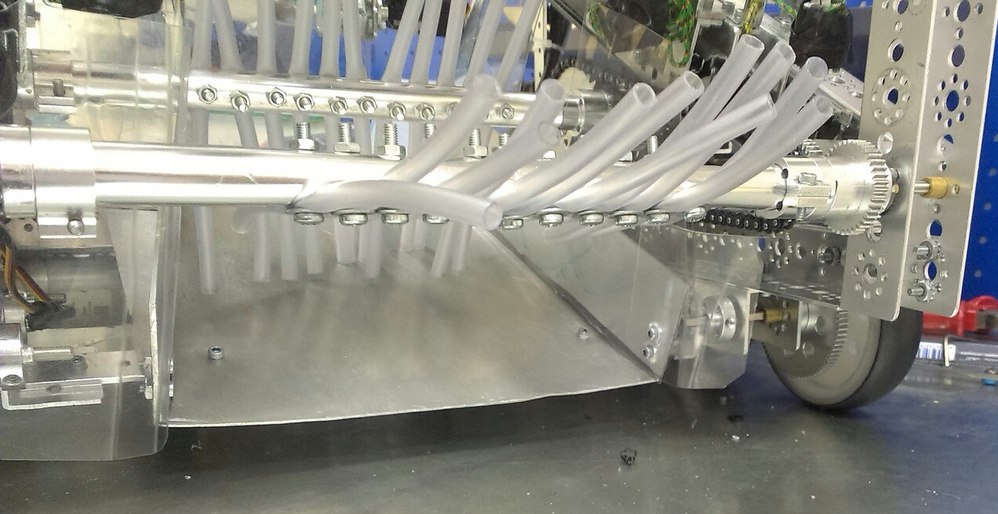
\includegraphics[scale=0.2]{3Engineering/5Team_meetings/days_of_meetings/2016.01.30/images/02}}
		\caption{Borders for debris (front)}
		\label{Gripper2.5}
	\end{minipage}
	\hfill
	\begin{minipage}[h]{0.47\linewidth}
		\center{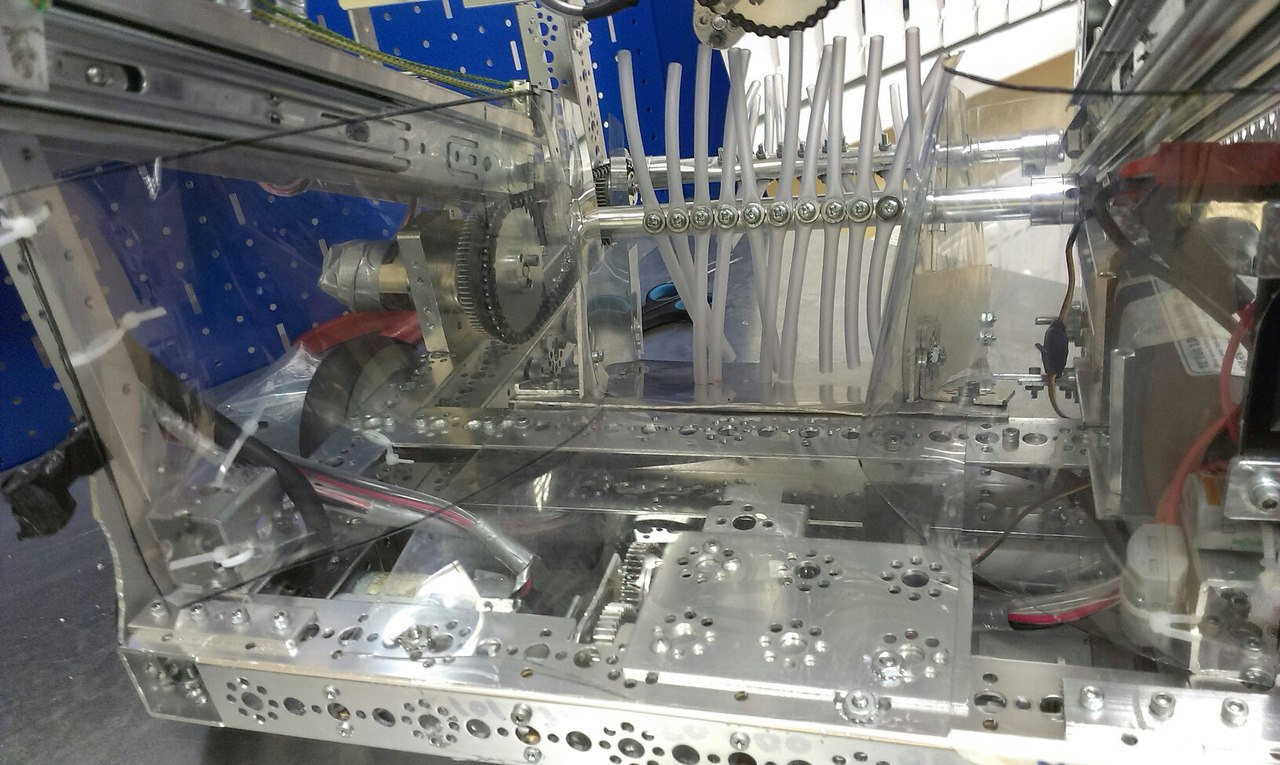
\includegraphics[scale=0.17]{3Engineering/5Team_meetings/days_of_meetings/2016.01.30/images/03}}
		\caption{Borders for debris (back)}
		\label{Gripper2.6}
	\end{minipage}
	\hfill
	\begin{minipage}[h]{0.47\linewidth}
		\center{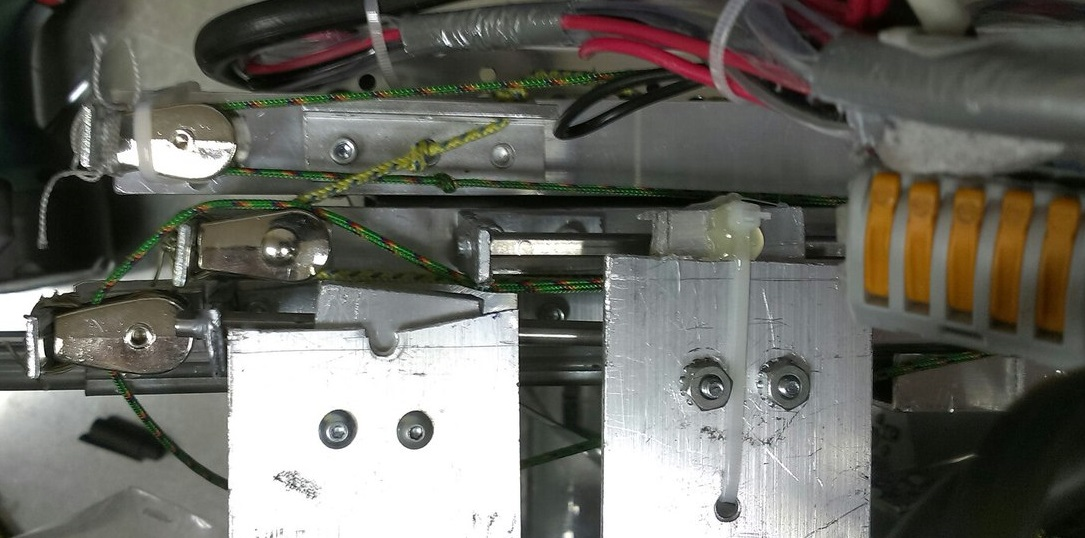
\includegraphics[scale=0.24]{3Engineering/5Team_meetings/days_of_meetings/2016.01.30/images/04}}
		\caption{The moving mounts of the ribs}
		\label{Elevator3.8}
	\end{minipage}
\end{figure}

The protection of the servos' wires on the bucket from grasping the elements of construction was finished. This protection will prevent wires from getting to the areas where it can get stuck (figure \ref{Shiftbuc2.13}, \ref{Shiftbuc2.14}).

\begin{figure}[H]
	\begin{minipage}[h]{0.47\linewidth}
		\center{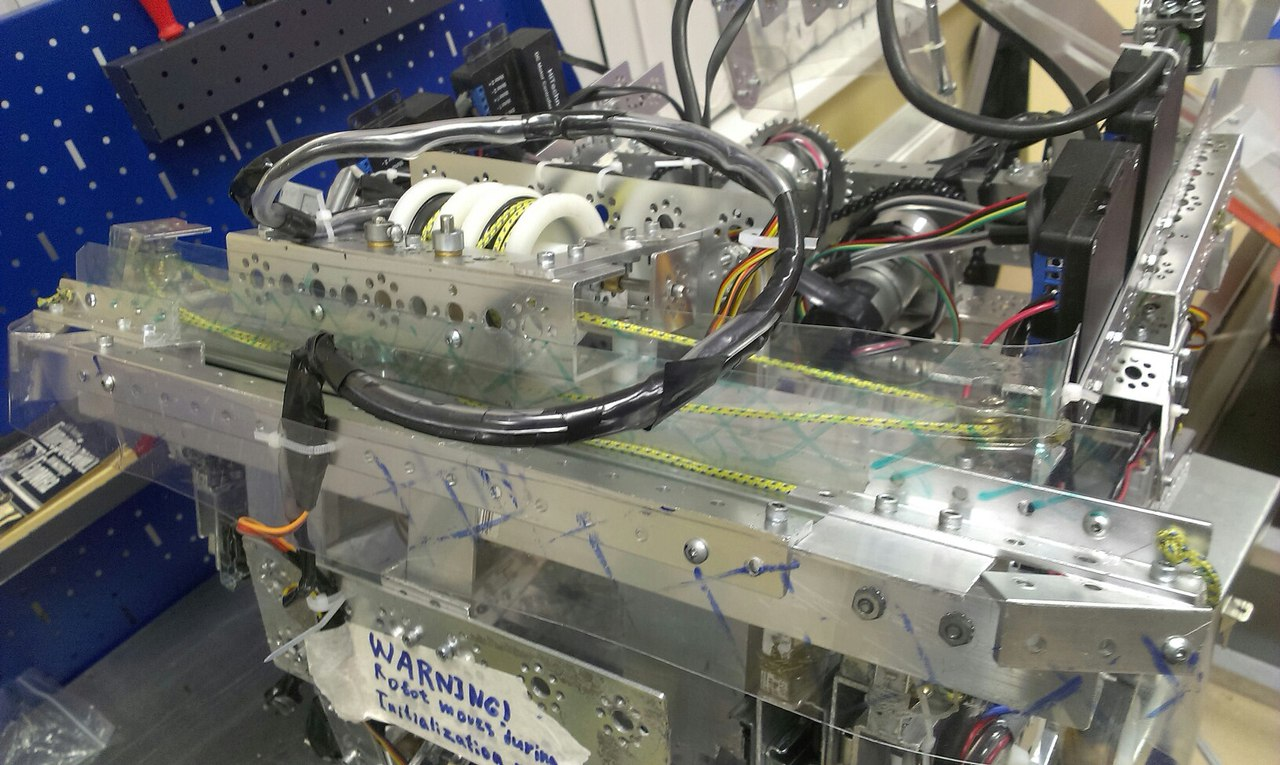
\includegraphics[scale=0.2]{3Engineering/5Team_meetings/days_of_meetings/2016.01.30/images/05}}
		\caption{Protection for wire}
		\label{Shiftbuc2.13}
	\end{minipage}
	\hfill
	\begin{minipage}[h]{0.47\linewidth}
		\center{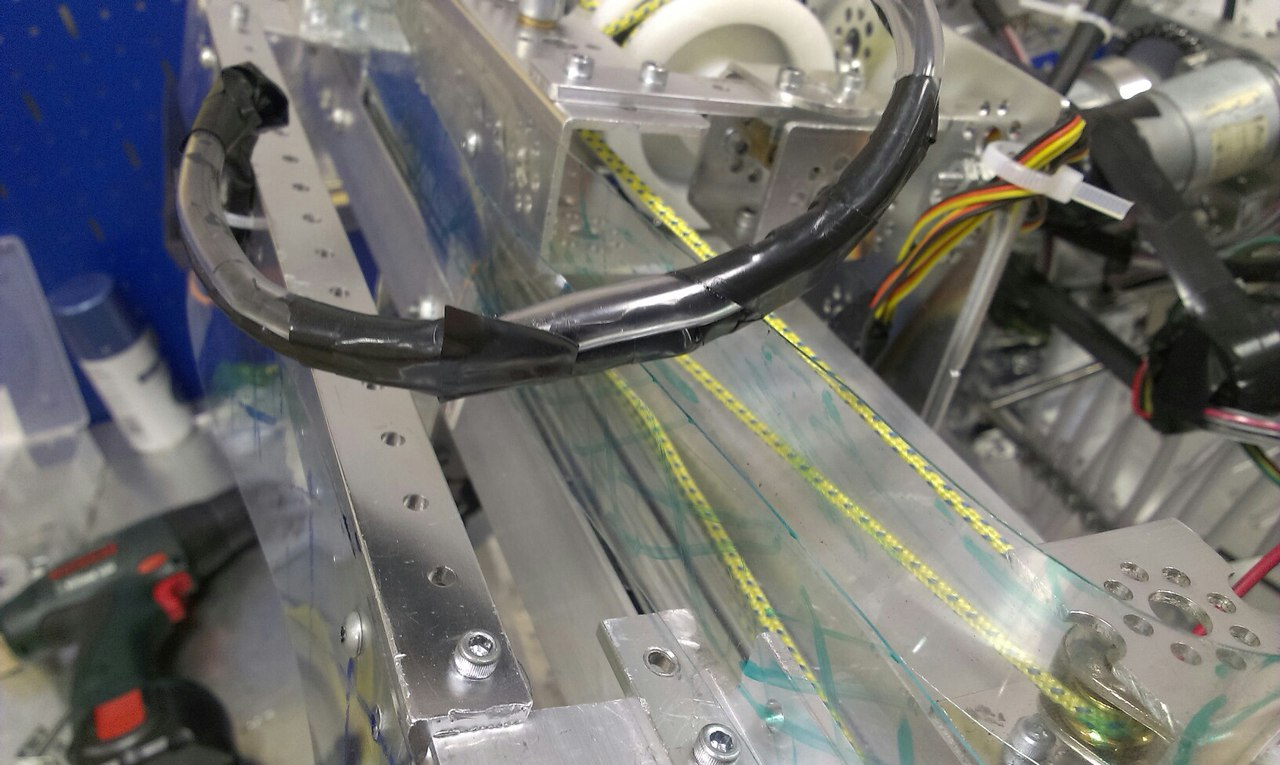
\includegraphics[scale=0.2]{3Engineering/5Team_meetings/days_of_meetings/2016.01.30/images/06}}
		\caption{How does the protection works}
		\label{Shiftbuc2.14}
	\end{minipage}
\end{figure}

It was created a new bucket for debris. It's shape allowed to collect 5 cubes at once, but was more convenient, than the previous.

%\begin{figure}[H]
%	\begin{minipage}[h]{0.47\linewidth}
%		\center{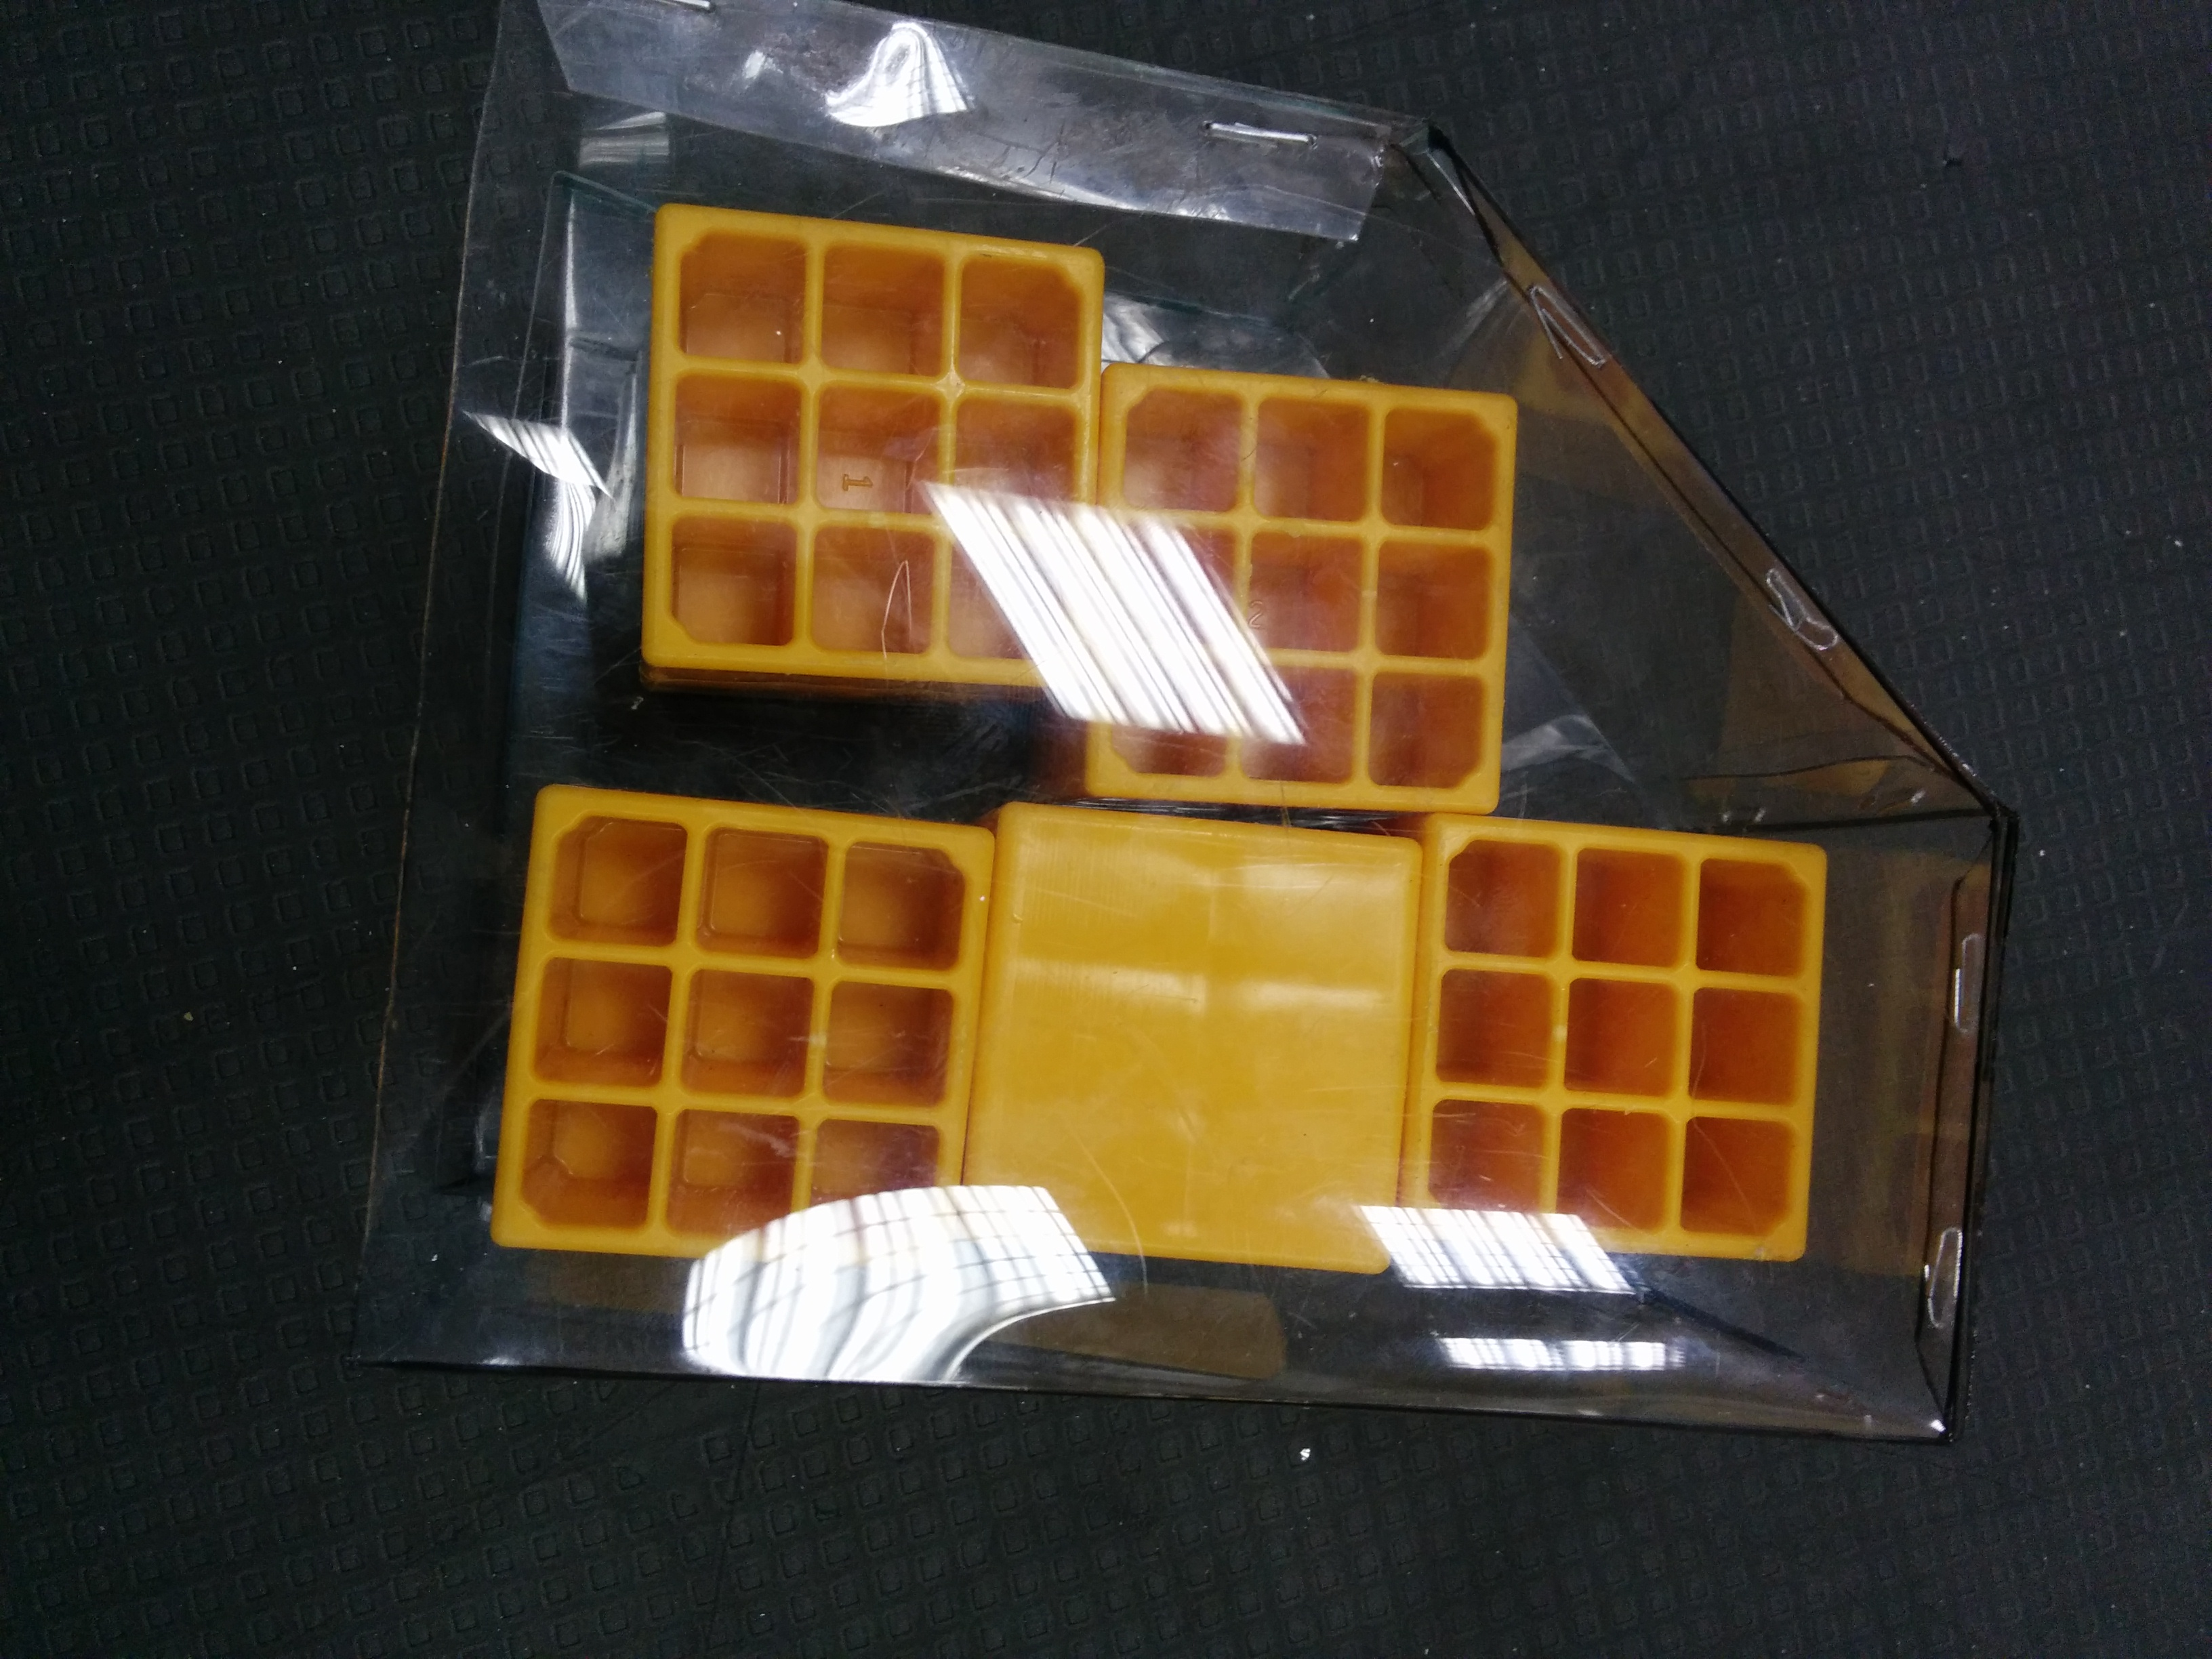
\includegraphics[scale=0.2]{3Engineering/5Team_meetings/days_of_meetings/2016.01.30/images/07}}
%		\caption{Bucket 1}
%	\end{minipage}
%	\hfill
%	\begin{minipage}[h]{0.47\linewidth}
%		\center{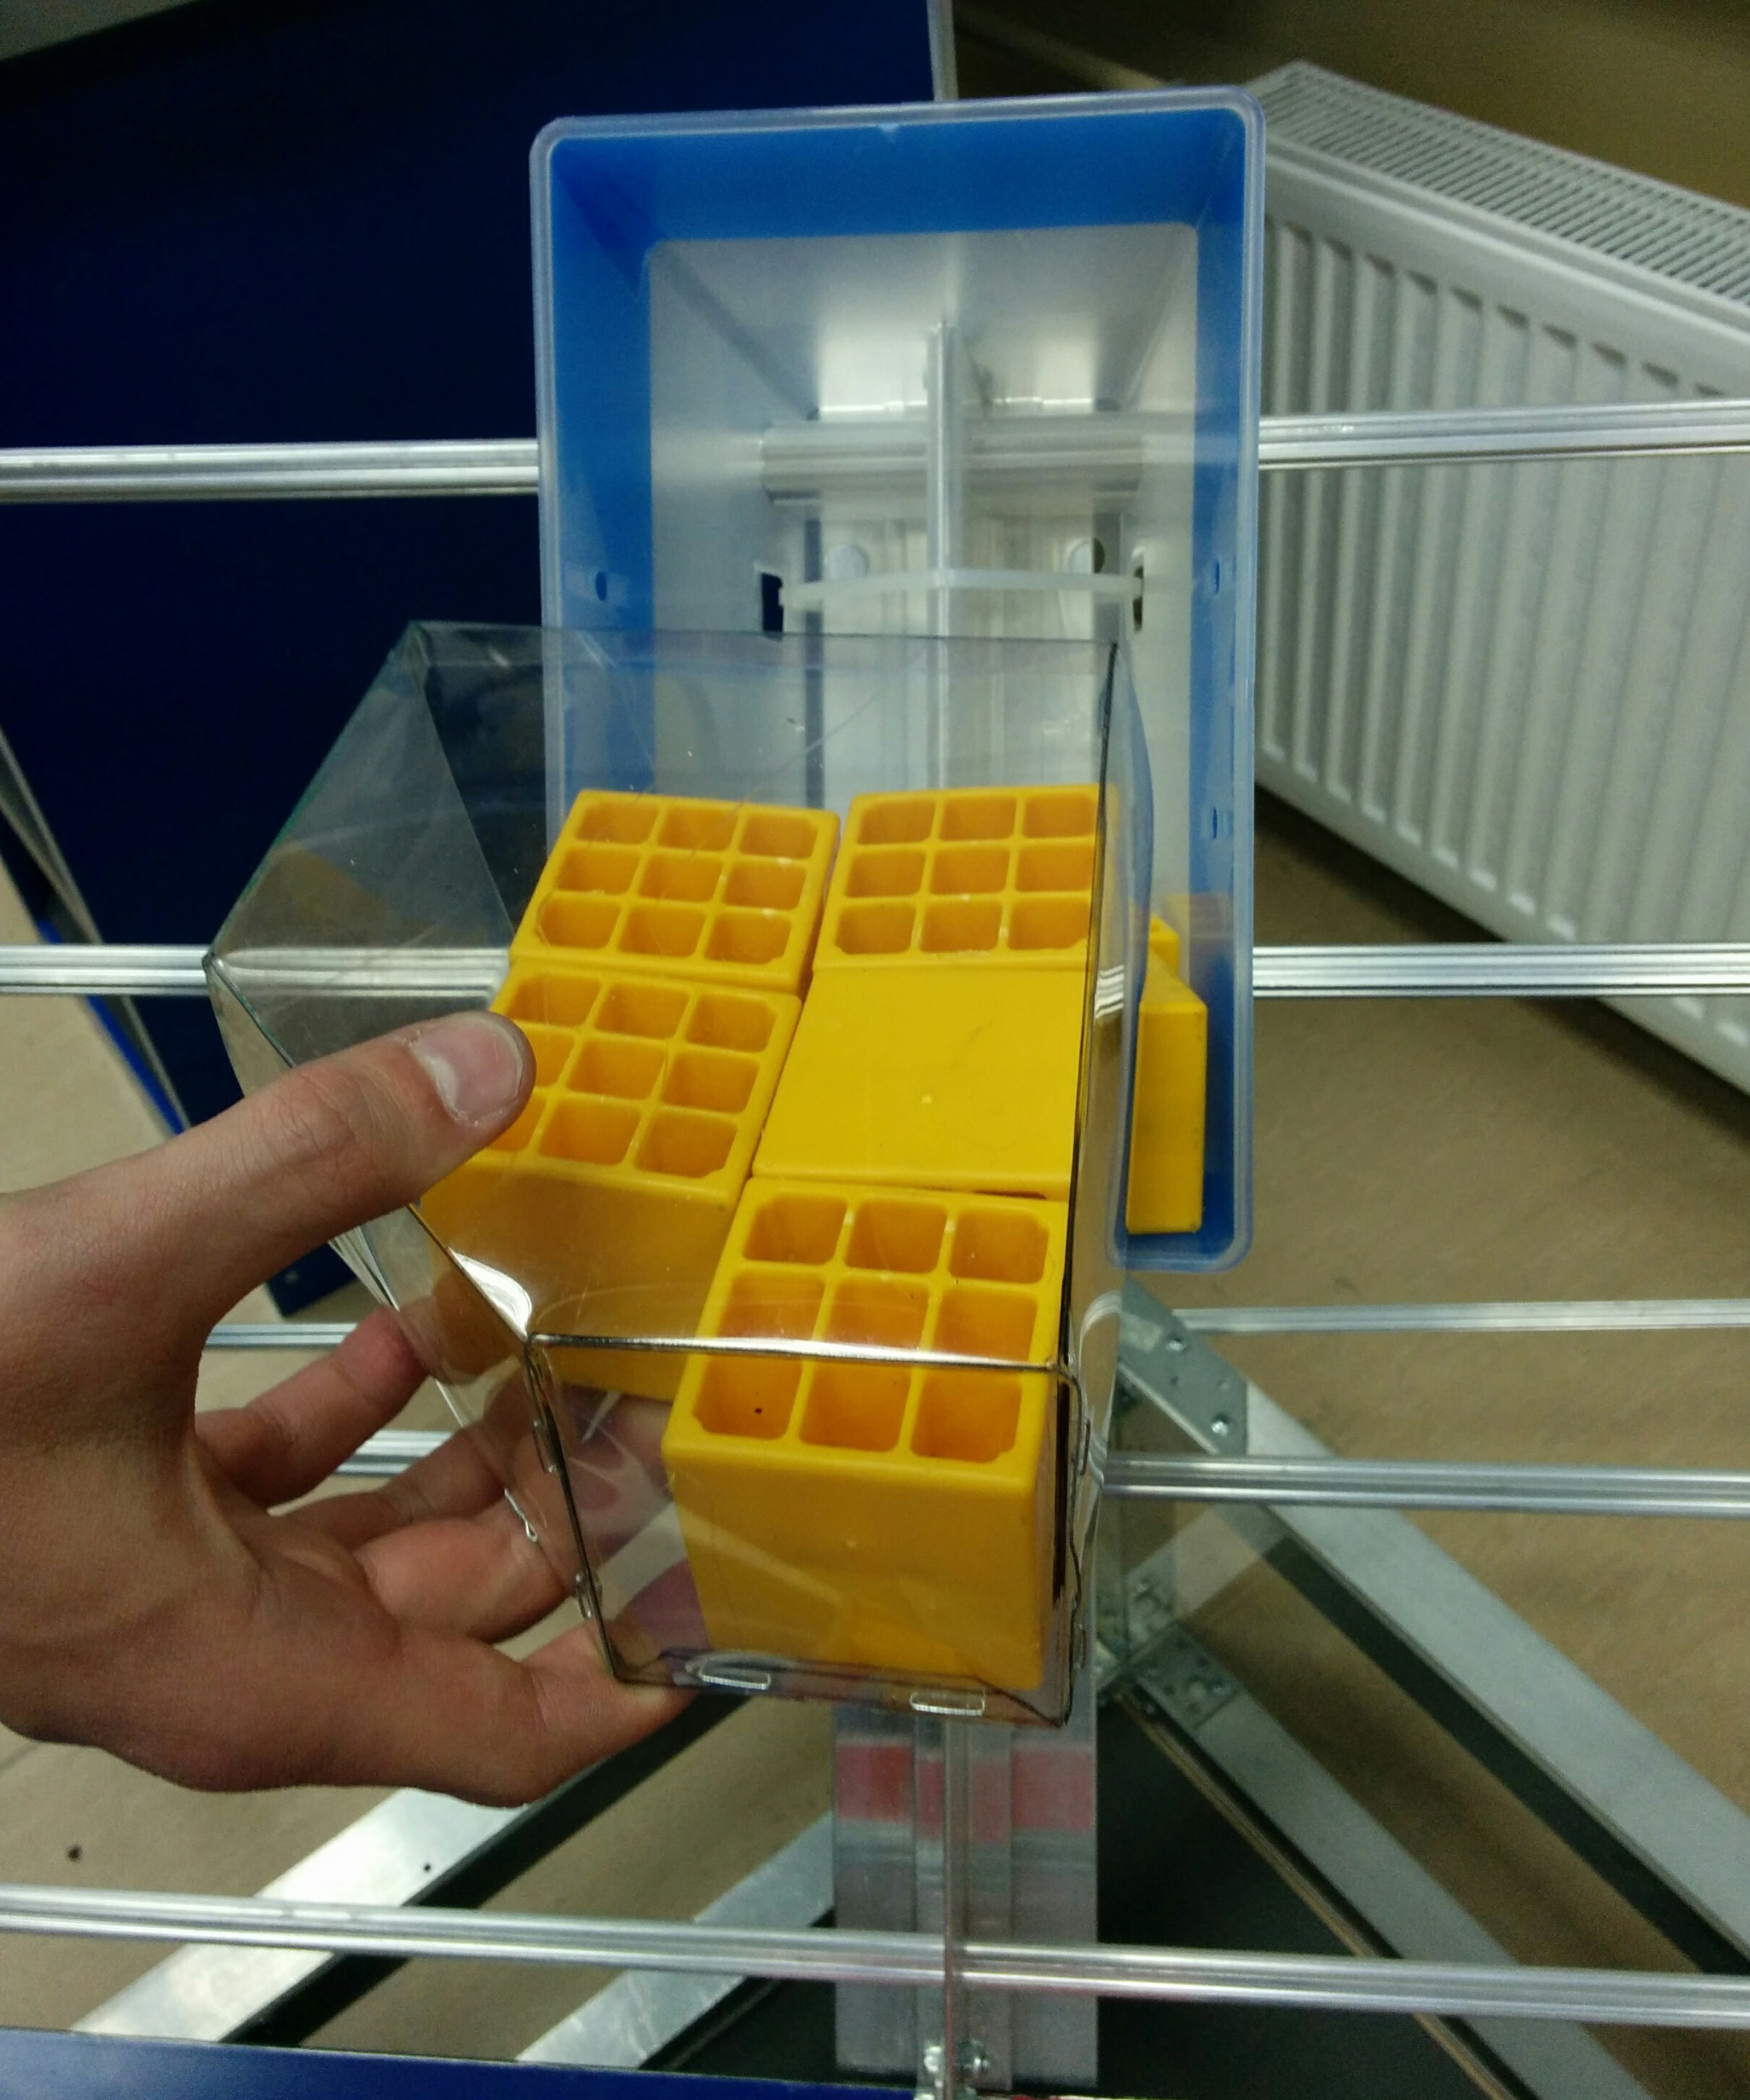
\includegraphics[scale=0.2]{3Engineering/5Team_meetings/days_of_meetings/2016.01.30/images/08}}
%		\caption{Bucket 2}
%	\end{minipage}
%\end{figure}
